\documentclass[tikz,border=10pt]{standalone}
\usepackage{mathrsfs}
\usepackage{physics}
\usetikzlibrary{decorations.pathmorphing}
    % this is for graphics. e.g. rectangle on title page
\usetikzlibrary{3d}
\usetikzlibrary{backgrounds}
\usetikzlibrary{arrows,shapes,positioning,shadows,trees,mindmap}
\usetikzlibrary{tikzmark}
\usetikzlibrary{calc,math}

\usepackage{tikz-3dplot}
\usepackage{pgfplots}
\pgfplotsset{compat = newest}
%\usepgfplotslibrary{colormaps}
\usepgflibrary{shapes.geometric}

\usepackage[edges]{forest}
\usetikzlibrary{arrows.meta}
\colorlet{linecol}{black!75}
\usepackage{xkcdcolors} % xkcd colors

\usetikzlibrary{patterns}
\tikzset{>={Stealth[inset=0pt,angle=20:10pt]}}


\tikzset{zigzag/.style={decorate,decoration=zigzag}}


\begin{document}
\tikzset{every picture/.style={line width=0.75pt}} %set default line width to 0.75pt        
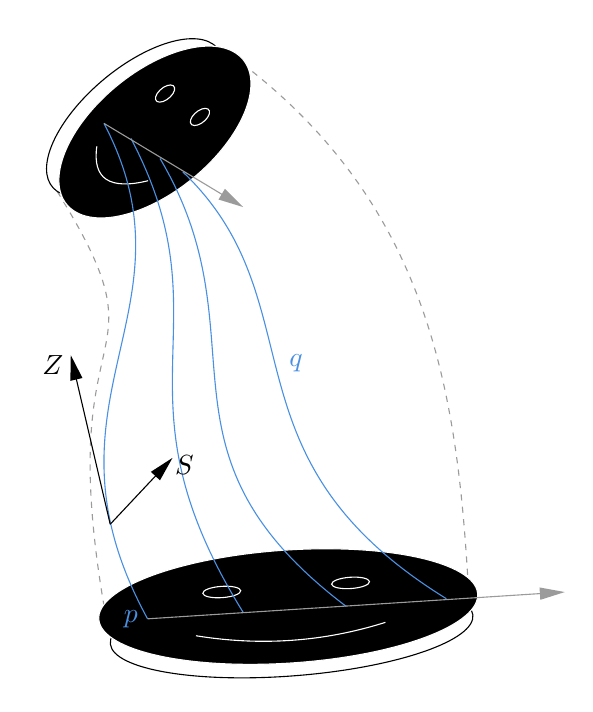
\begin{tikzpicture}[x=0.75pt,y=0.75pt,yscale=2.5,xscale=2.5]
%uncomment if require: \path (0,310); %set diagram left start at 0, and has height of 310

%Curve Lines [id:da7996812604575372] 
\draw [color={rgb, 255:red, 155; green, 155; blue, 155 }  ,draw opacity=1 ] [dash pattern={on 2.25pt off 2.25pt on 2.25pt off 2.25pt}]  (6.77,99.09) .. controls (29.4,62.67) and (4.6,78.8) .. (16.6,14.77) ;
%Curve Lines [id:da8260353134732461] 
\draw [color={rgb, 255:red, 155; green, 155; blue, 155 }  ,draw opacity=1 ] [dash pattern={on 2.25pt off 2.25pt on 2.25pt off 2.25pt}]  (40.6,125.09) .. controls (78.2,97.35) and (83.8,61.22) .. (86,23.11) ;
%Shape: Ellipse [id:dp6289187782802004] 
\draw   (36.83,127.44) .. controls (41.3,124.35) and (38.2,115.51) .. (29.89,107.68) .. controls (21.59,99.85) and (11.24,96.01) .. (6.77,99.09) .. controls (2.3,102.17) and (5.41,111.02) .. (13.71,118.84) .. controls (22.01,126.67) and (32.36,130.52) .. (36.83,127.44) -- cycle ;
%Shape: Ellipse [id:dp336692845921404] 
\draw   (17.03,11.81) .. controls (16.42,16.72) and (31.56,21.97) .. (50.85,23.54) .. controls (70.14,25.1) and (86.28,22.4) .. (86.89,17.49) .. controls (87.5,12.59) and (72.36,7.34) .. (53.07,5.77) .. controls (33.78,4.2) and (17.64,6.9) .. (17.03,11.81) -- cycle ;
%Shape: Smiley Face [id:dp3137449331689346] 
\draw  [color={rgb, 255:red, 255; green, 255; blue, 255 }  ,draw opacity=1 ][fill={rgb, 255:red, 0; green, 0; blue, 0 }  ,fill opacity=1 ] (14.81,16.49) .. controls (14.16,22.47) and (29.97,28.47) .. (50.13,29.9) .. controls (70.29,31.32) and (87.16,27.62) .. (87.81,21.64) .. controls (88.46,15.66) and (72.64,9.65) .. (52.49,8.23) .. controls (32.33,6.81) and (15.46,10.5) .. (14.81,16.49) -- cycle ; \draw  [color={rgb, 255:red, 255; green, 255; blue, 255 }  ,draw opacity=1 ][fill={rgb, 255:red, 0; green, 0; blue, 0 }  ,fill opacity=1 ] (34.85,21.61) .. controls (34.78,22.21) and (36.37,22.81) .. (38.38,22.95) .. controls (40.4,23.1) and (42.08,22.73) .. (42.15,22.13) .. controls (42.21,21.53) and (40.63,20.93) .. (38.62,20.79) .. controls (36.6,20.64) and (34.91,21.01) .. (34.85,21.61) -- cycle ; \draw  [color={rgb, 255:red, 255; green, 255; blue, 255 }  ,draw opacity=1 ][fill={rgb, 255:red, 0; green, 0; blue, 0 }  ,fill opacity=1 ] (59.67,23.37) .. controls (59.6,23.96) and (61.18,24.56) .. (63.2,24.71) .. controls (65.21,24.85) and (66.9,24.48) .. (66.97,23.88) .. controls (67.03,23.28) and (65.45,22.68) .. (63.43,22.54) .. controls (61.42,22.4) and (59.73,22.77) .. (59.67,23.37) -- cycle ; \draw  [color={rgb, 255:red, 255; green, 255; blue, 255 }  ,draw opacity=1 ] (33.53,13.44) .. controls (46.01,11.41) and (58.18,12.27) .. (70.03,16.02) ;
%Shape: Smiley Face [id:dp518617277802321] 
\draw  [color={rgb, 255:red, 255; green, 255; blue, 255 }  ,draw opacity=1 ][fill={rgb, 255:red, 0; green, 0; blue, 0 }  ,fill opacity=1 ] (15.73,117.14) .. controls (24.37,125.53) and (35.8,129.35) .. (41.26,125.69) .. controls (46.72,122.03) and (44.14,112.27) .. (35.5,103.89) .. controls (26.86,95.51) and (15.43,91.68) .. (9.97,95.34) .. controls (4.51,99) and (7.09,108.76) .. (15.73,117.14) -- cycle ; \draw  [color={rgb, 255:red, 255; green, 255; blue, 255 }  ,draw opacity=1 ][fill={rgb, 255:red, 0; green, 0; blue, 0 }  ,fill opacity=1 ] (26.59,118.59) .. controls (27.45,119.43) and (28.59,119.81) .. (29.14,119.45) .. controls (29.68,119.08) and (29.43,118.11) .. (28.56,117.27) .. controls (27.7,116.43) and (26.56,116.05) .. (26.01,116.41) .. controls (25.46,116.78) and (25.72,117.75) .. (26.59,118.59) -- cycle ; \draw  [color={rgb, 255:red, 255; green, 255; blue, 255 }  ,draw opacity=1 ][fill={rgb, 255:red, 0; green, 0; blue, 0 }  ,fill opacity=1 ] (33.31,114.09) .. controls (34.17,114.93) and (35.32,115.31) .. (35.86,114.94) .. controls (36.41,114.58) and (36.15,113.6) .. (35.29,112.76) .. controls (34.42,111.92) and (33.28,111.54) .. (32.73,111.91) .. controls (32.19,112.27) and (32.44,113.25) .. (33.31,114.09) -- cycle ; \draw  [color={rgb, 255:red, 255; green, 255; blue, 255 }  ,draw opacity=1 ] (14.42,107.76) .. controls (13.54,101.51) and (16.83,99.3) .. (24.3,101.13) ;
%Curve Lines [id:da6520443256492074] 
\draw [color={rgb, 255:red, 74; green, 144; blue, 226 }  ,draw opacity=1 ]   (15.8,112.18)  .. controls (34.8,75.89) and (1.2,58.84) .. (24.2,16.7) node[left]{$p$};
%Curve Lines [id:da29091903800222285] 
\draw [color={rgb, 255:red, 74; green, 144; blue, 226 }  ,draw opacity=1 ]   (21,109.28) .. controls (40,72.99) and (16.2,60.57) .. (42.6,17.99) ;
%Curve Lines [id:da32452590534719583] 
\draw [color={rgb, 255:red, 74; green, 144; blue, 226 }  ,draw opacity=1 ]   (26.6,105.41) .. controls (47,70.89) and (23,48.96) .. (62.5,19.08) ;
%Curve Lines [id:da8986334447857889] 
\draw [color={rgb, 255:red, 74; green, 144; blue, 226 }  ,draw opacity=1 ]   (31,102.83) .. controls (57.5,77.43) and (37.3,47.99) .. (81.8,20.57) node[midway,above right]{$q$};
%Straight Lines [id:da2931926297199059] 
\draw    (17,34.93) -- (9.85,65.56) node[left]{$Z$};
\draw [shift={(9.4,67.51)}, rotate = 283.13] [fill={rgb, 255:red, 0; green, 0; blue, 0 }  ][line width=0.08]  [draw opacity=0] (4.8,-1.2) -- (0,0) -- (4.8,1.2) -- cycle    ;
%Straight Lines [id:da5411972145491839] 
\draw    (17,34.93) -- (27.63,46.25) node[right]{$S$};
\draw [shift={(29,47.71)}, rotate = 226.81] [fill={rgb, 255:red, 0; green, 0; blue, 0 }  ][line width=0.08]  [draw opacity=0] (4.8,-1.2) -- (0,0) -- (4.8,1.2) -- cycle    ;
%Straight Lines [id:da2346032603024848] 
\draw [color={rgb, 255:red, 155; green, 155; blue, 155 }  ,draw opacity=1 ]   (24.2,16.7) -- (102.6,21.74);
\draw [shift={(104.6,21.86)}, rotate = 183.67] [fill={rgb, 255:red, 155; green, 155; blue, 155 }  ,fill opacity=1 ][line width=0.08]  [draw opacity=0] (4.8,-1.2) -- (0,0) -- (4.8,1.2) -- cycle    ;
%Straight Lines [id:da7594891715610954] 
\draw [color={rgb, 255:red, 155; green, 155; blue, 155 }  ,draw opacity=1 ]   (15.8,112.18) -- (40.89,97.09) ;
\draw [shift={(42.6,96.06)}, rotate = 148.96] [fill={rgb, 255:red, 155; green, 155; blue, 155 }  ,fill opacity=1 ][line width=0.08]  [draw opacity=0] (4.8,-1.2) -- (0,0) -- (4.8,1.2) -- cycle    ;
\end{tikzpicture}
\end{document}